\documentclass{beamer}
\usetheme[sectionpage=none]{metropolis}
%\usepackage[backend=biber]{biblatex}
%\usepackage{booktabs} 
\usepackage{url}
\def\UrlBreaks{\do\/\do-}
\usepackage{amsfonts, amsmath, lmodern}
\usefonttheme{serif}
\usepackage{algorithm}
\usepackage{algorithmic}


%plots
\usepackage{tikz}
\usepackage{pgfplots}
\usepackage{pgfplotstable}
\pgfplotsset{compat=newest}
\usepackage{subcaption}
\usepackage{csvsimple}
%bibliography numbers
\setbeamertemplate{bibliography item}{\insertbiblabel}

\graphicspath{{./pictures}}
\setbeameroption{show notes} % comment out for the real presentation

\title{Fast Search of the Optimal Contraction Sequence in Tensor Networks}

\author{Max Koch, Christian Ortlepp}


\institute{Friedrich-Schiller-Universität Jena}

\date{20. Januar 2023}




\begin{document}

\begin{frame}
	\titlepage
  \end{frame}

\begin{frame}{Gliederung}
	\tableofcontents
\end{frame}

\section{Einführung und Zielsetzung}
\begin{frame}{Einführung}
	TBD
\end{frame}

\section{Tensor-Kontraktionen}

\begin{frame}{Begriffseinführungen}
	\begin{columns}
		\begin{column}{0.5\textwidth}
			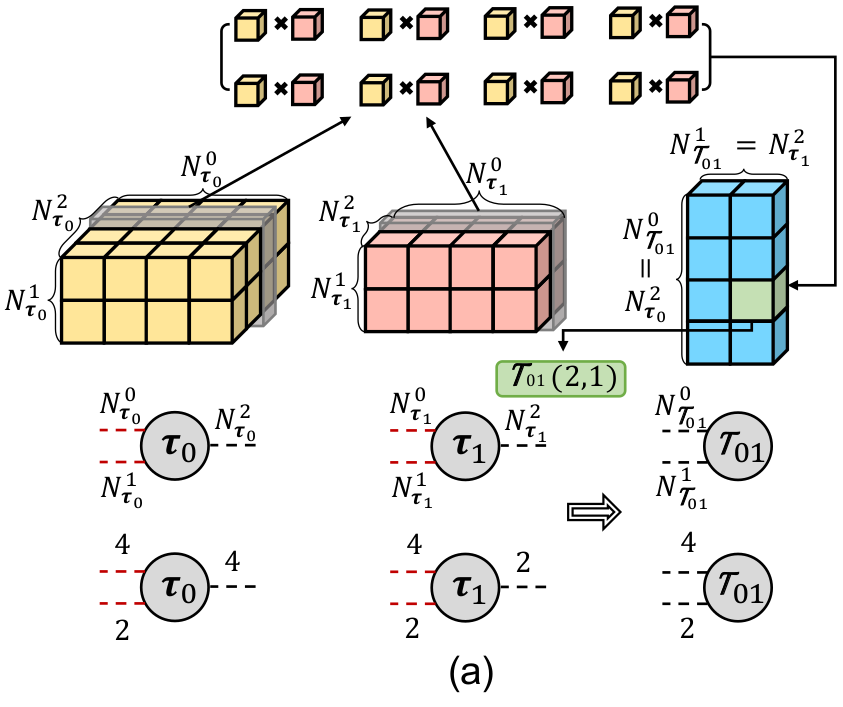
\includegraphics[scale=.2]{figure-2-a}
		\end{column}
		\begin{column}{0.5\textwidth}
			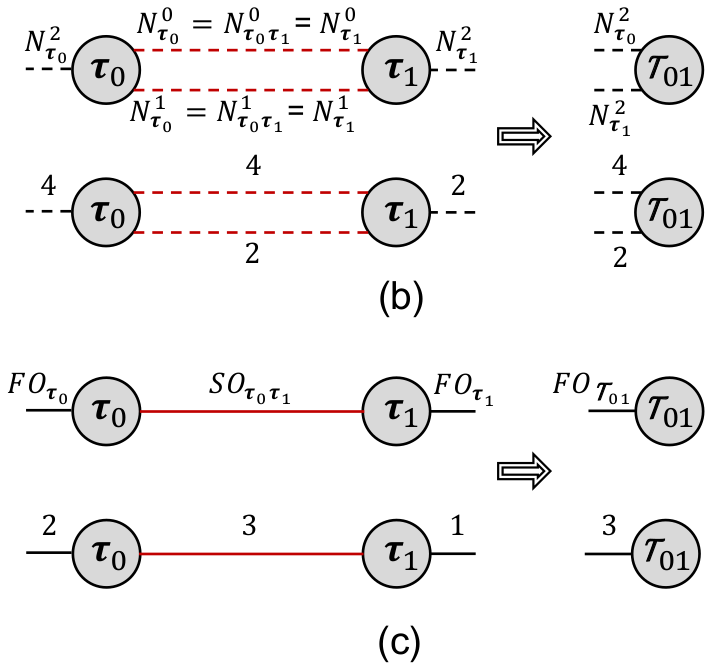
\includegraphics[scale=.2]{figure-2-b}
		\end{column}
	\end{columns}
\end{frame}
\note[itemize]{
\item Graph-Notation: Kanten=Dimensionen (Order), Knoten=Tensoren
\item Kanten zwischen Knoten "Sharing Orders", sonst "Free Orders"
\item Kantengewicht: $\log_2$ der Order
\item bei $V$ Tensoren werden $V-1$ Schritte benötigt
}

\begin{frame}{Kontraktion}
	\begin{columns}
		\begin{column}{0.5\textwidth}
			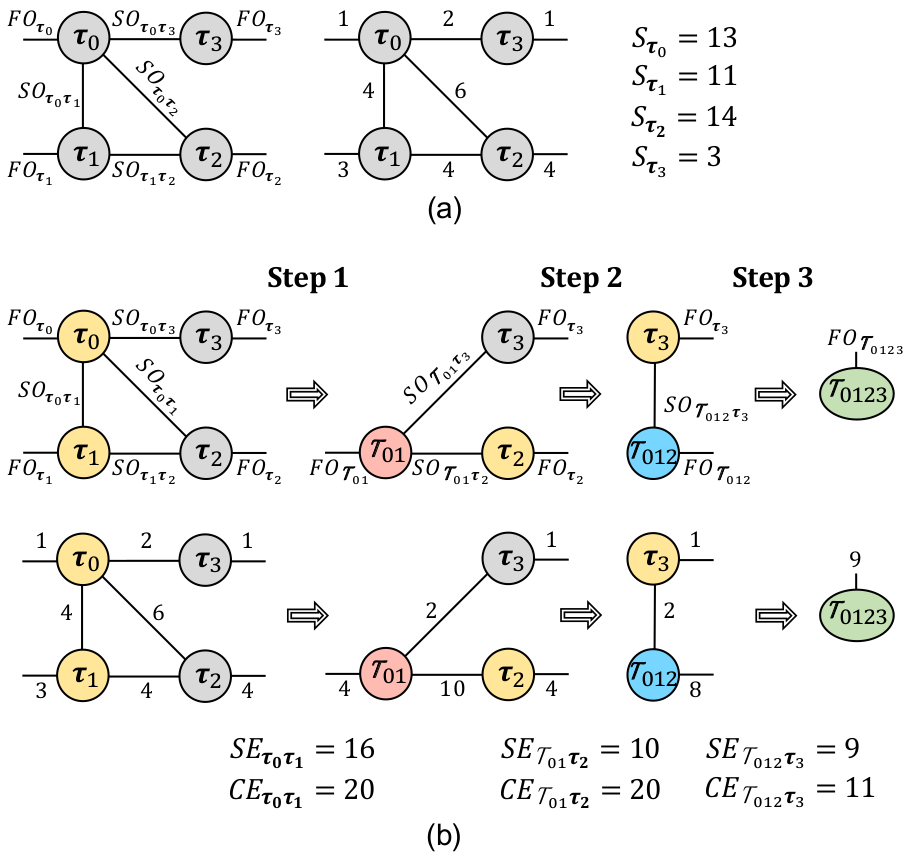
\includegraphics[scale=.17]{figure-3-a}
		\end{column}
		\begin{column}{0.5\textwidth}
			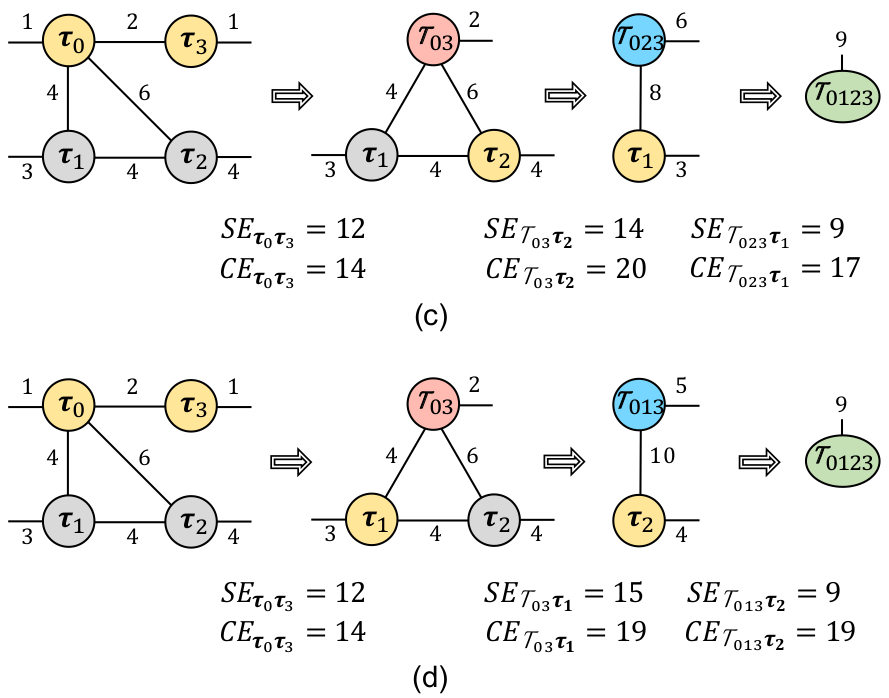
\includegraphics[scale=.17]{figure-3-b}
		\end{column}
	\end{columns}
\end{frame}
\note[itemize]{
\item verschiedene Kontraktionsreihenfolgen
\item bei jedem schritt wird eine sharing order eliminiert
}


\begin{frame}[allowframebreaks]{Bibliography}
	\bibliography{../bibliography/bibliography.bib}
	\bibliographystyle{splncs04}
\end{frame}

\end{document}
